\documentclass[fleqn, 11pt]{article}

\usepackage{verbatim}
\usepackage{amsmath}
\usepackage{amssymb}
\usepackage{amsthm}
\usepackage{hyperref}
\usepackage{ulem}
\usepackage{enumitem}
\usepackage[top=1.0in, left=0.75in, right=0.75in, bottom=0.75in]{geometry}
\usepackage{graphicx}
\usepackage{subcaption}

\newcommand{\myline}{
    \par
    \kern3pt % space above the rules
    \hrule height 0.5pt
    \kern2pt % space between the rules
    \hrule height 0.5pt
    \kern3pt % space below the rules
    \par
}

\usepackage[T1]{fontenc}

\usepackage{array}
\usepackage{caption}
\usepackage{floatrow}
\usepackage{multirow}

\usepackage{chngcntr}
\counterwithin*{equation}{section}

\usepackage{sectsty}
\sectionfont{\centering}

\usepackage[perpage]{footmisc}

\usepackage{fancyhdr}
\pagestyle{fancy}
\fancyhf{}
\lhead{190100036 \& 190100044}
\rhead{SI424: Project}
\renewcommand{\footrulewidth}{1.0pt}
\cfoot{Page \thepage}

\setlength{\parindent}{0em}
\renewcommand{\arraystretch}{2}

\title{SI 424: Statistical Inference \\ Project Report}
\author{
    \begin{tabular}{|c|c|}
        \hline
        \textsf{Krushnakant Bhattad} & \textsf{ \hspace{5pt} Devansh Jain \hspace{5pt} } \\
        \hline
        \textsf{190100036} & \textsf{190100044}\\
        \hline
    \end{tabular}
}
\date{Autumn 2021}

\begin{document}

\maketitle
\thispagestyle{empty}
\renewcommand{\arraystretch}{1}%
\setcounter{page}{0}

\myline
\vspace{10pt}
\underline{\large {\textsc{Project Title}}}:

\medskip

Experiments on Parameter Estimation and Hypothesis Testing

\vspace{7pt}
\myline
\vspace{10pt}
\underline{\large {\textsc{Abstract}}}:

\medskip

We first devise two problems on parameter estimation. We perform experiments for different sample size and observe the varied value of estimates.

We also devise two problems on hypothesis testing. We perform experiments for different sample size and different true values and observe the variation in Type I error and Type II error.

\vspace{7pt}
\myline
\vspace{10pt}
\underline{\large {\textsc{Associated GitHub Repository}}}:

\medskip

The GitHub repository can accessed at: \url{https://github.com/devansh-dvj/SI424-Project}

\vspace{7pt}
\myline
\vspace{10pt}
\underline{\large {\textsc{Common Notations}}}:

\medskip

$\mathcal{N}(\mu, \sigma^2)$ denotes the Normal distribution with mean $\mu$ and variance $\sigma^2$. \\
$\mathrm{Binomial}(p, n)$ denotes the Binomial distribution with probability of success $p$ and number of trials $n$. \\
$\mathrm{Uniform}[\theta_1, \theta_2]$ denotes the Uniform distribution with lower bound $\theta_1$ and upper bound $\theta_2$. \\
$\mathrm{mean}(x)$ denotes mean of elements in vector $x$. \\
$\mathrm{max}(x)$ denotes maximum of elements in vector $x$. \\
$\mathrm{min}(x)$ denotes minimum of elements in vector $x$.

\vspace{7pt}
\myline


\newpage
\section{Parameter estimation Problem 1}
\setcounter{figure}{0}
\subsection{Analysis of Population Growth Rate}
\begin{figure}[H]
    \centering
    \begin{subfigure}[H]{0.49\textwidth}
        \centering
        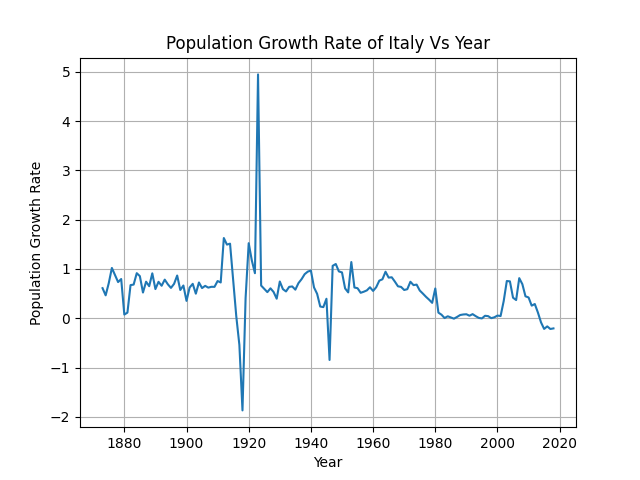
\includegraphics[width=\textwidth]{P1/plot.png}
        \caption[]{Plot of Population Growth Rate of Italy Vs Year}
    \end{subfigure}
    \begin{subfigure}[H]{0.49\textwidth}
        \centering
        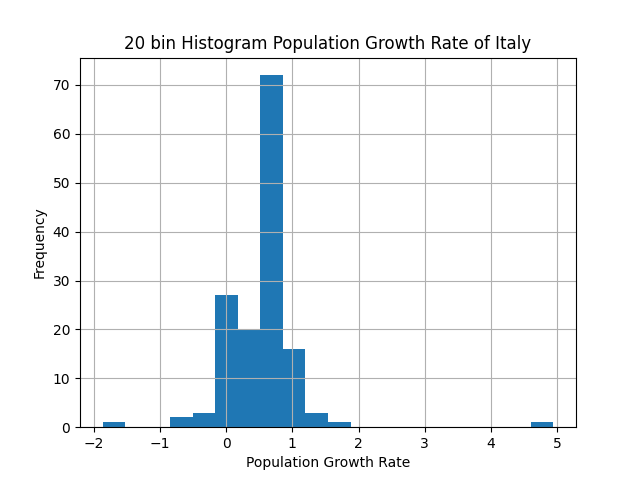
\includegraphics[width=\textwidth]{P1/hist.png}
        \caption[]{Histogram of Population Growth Rate of Italy}
    \end{subfigure}
    \caption{Analysis of Population Growth Rate of Italy}
\end{figure}

From the above obtained plot and histogram, we can approximate population growth rate of Italy as a constant $\mu$ with zero-mean additive Gaussian noise, i.e. population growth rate of Italy $\sim \mathcal{N}(\mu, \sigma^2)$. \\

\subsection{Problem Description}
We assume that the population growth rate of Italy follows $\mathcal{N}(\mu, \sigma^2)$ distribution. \\
We are given a sample of population growth rate $g = (g_1, \dots, g_K)$ where $K$ is the sample size. \\
Estimated values are $\hat{\mu}_{MLE} = \mathrm{mean}(g)$ and $\hat{\sigma}_{MLE} = \sqrt{ \mathrm{mean}((g - \hat{\mu}_{MLE})^2) }$. \\
We perform this experiment for $N$ iterations for a fixed $K$. \\
We analyze the observed estimated of $\mu$ and $\sigma$ for different $K$ and $N$. \\

\subsection{Generation of Sample}
From \verb!population_Country.csv!, we determine year-wise population growth rate for Italy from 1872 to 2018 (list of size 147). \\
The population growth rates are computed as percentage change in population (using \verb!Total2! column) for every year. \\
Our $K$-sized sample is a randomly chosen $K$-sized subset $(K \le 147)$ of the above obtained list. \\
We use function \verb!numpy.random.choice! with suitable arguments to obtain this sample. \\

\subsection{Results}
\subsubsection{Estimate of $\mu$}
\begin{figure}[H]
    \centering
    \begin{subfigure}[H]{0.49\textwidth}
        \centering
        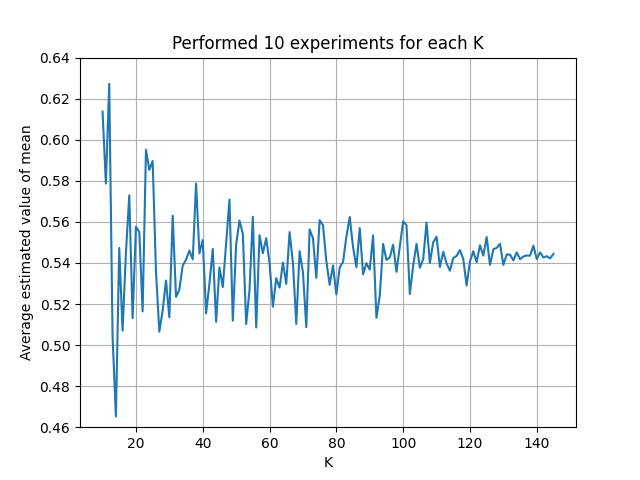
\includegraphics[width=\textwidth]{P1/mu/avgs_10.png}
        \caption[]{Average value of $\hat{\mu}_{MLE}$ observed}
    \end{subfigure}
    \begin{subfigure}[H]{0.49\textwidth}
        \centering
        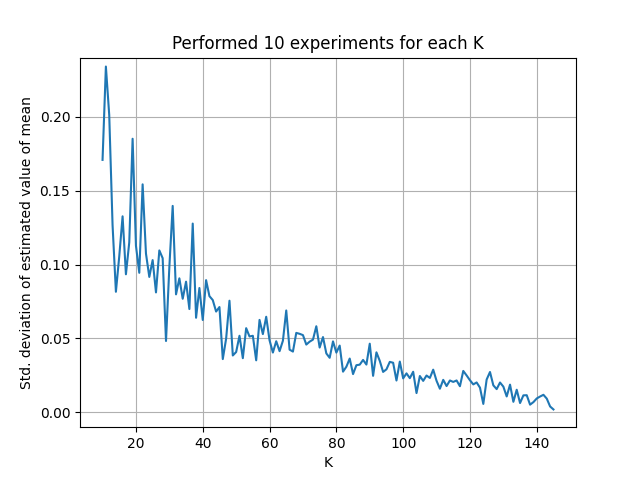
\includegraphics[width=\textwidth]{P1/mu/stds_10.png}
        \caption[]{Std. deviation of $\hat{\mu}_{MLE}$ observed}
    \end{subfigure}
    \caption{Number of iterations, $N = 10$}
\end{figure}
\vspace{30pt}
\begin{figure}[H]
    \centering
    \begin{subfigure}[H]{0.49\textwidth}
        \centering`
        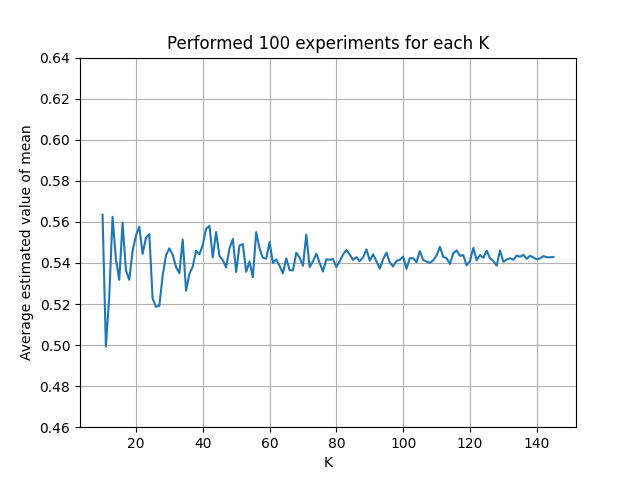
\includegraphics[width=\textwidth]{P1/mu/avgs_100.png}
        \caption[]{Average value of $\hat{\mu}_{MLE}$ observed}
    \end{subfigure}
    \begin{subfigure}[H]{0.49\textwidth}
        \centering
        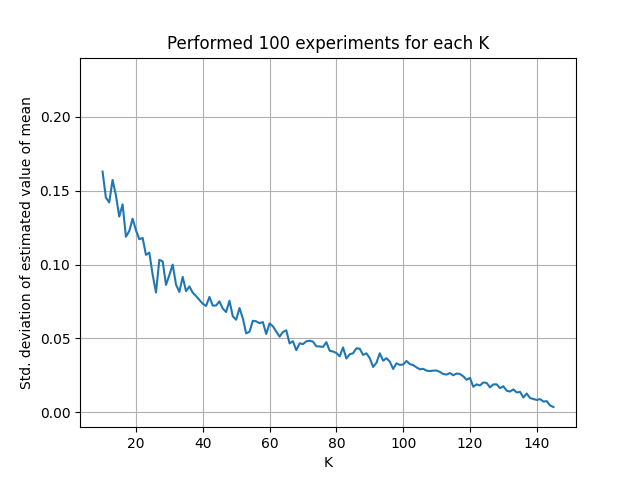
\includegraphics[width=\textwidth]{P1/mu/stds_100.png}
        \caption[]{Std. deviation of $\hat{\mu}_{MLE}$ observed}
    \end{subfigure}
    \caption{Number of iterations, $N = 100$}
\end{figure}
\newpage
\begin{figure}[H]
    \centering
    \begin{subfigure}[H]{0.49\textwidth}
        \centering
        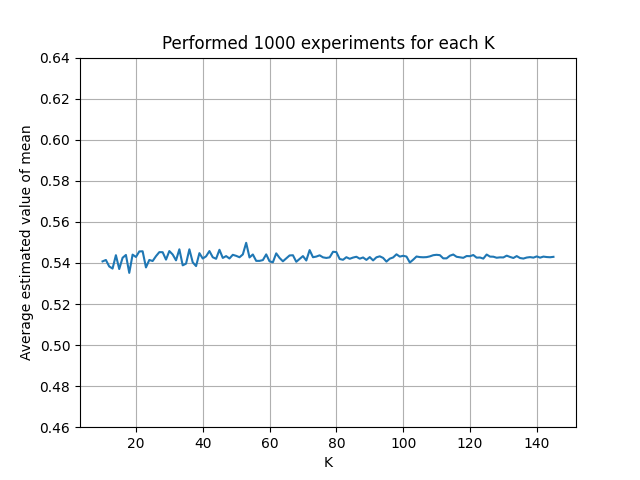
\includegraphics[width=\textwidth]{P1/mu/avgs_1000.png}
        \caption[]{Average value of $\hat{\mu}_{MLE}$ observed}
    \end{subfigure}
    \begin{subfigure}[H]{0.49\textwidth}
        \centering
        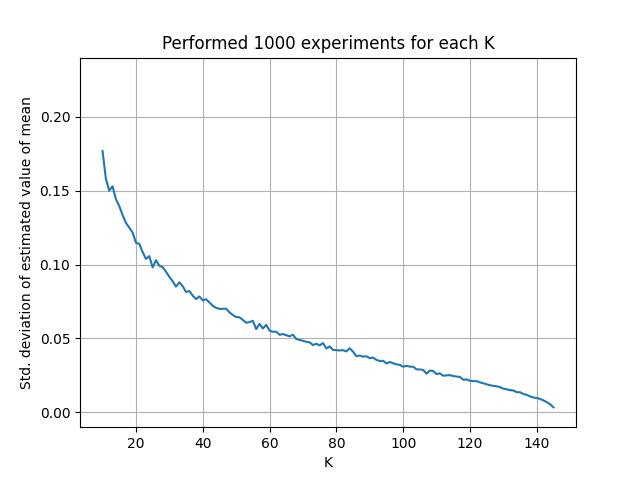
\includegraphics[width=\textwidth]{P1/mu/stds_1000.png}
        \caption[]{Std. deviation of $\hat{\mu}_{MLE}$ observed}
    \end{subfigure}
    \caption{Number of iterations, $N = 1000$}
\end{figure}
\vspace{30pt}
\subsubsection{Estimate of $\sigma$}
\begin{figure}[H]
    \centering
    \begin{subfigure}[H]{0.49\textwidth}
        \centering
        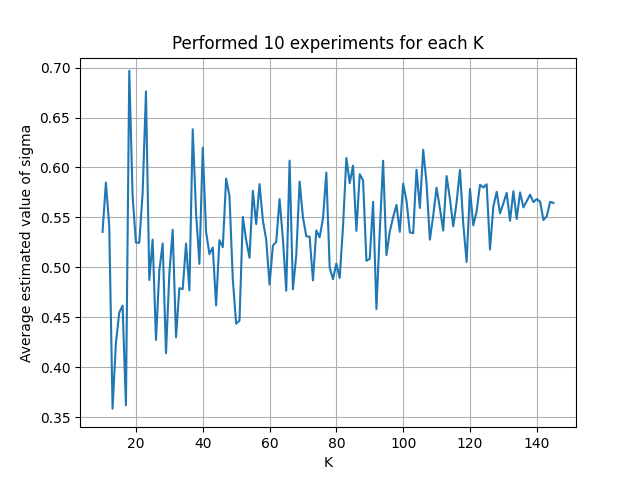
\includegraphics[width=\textwidth]{P1/sigma/avgs_10.png}
        \caption[]{Average value of $\hat{\sigma}_{MLE}$ observed}
    \end{subfigure}
    \begin{subfigure}[H]{0.49\textwidth}
        \centering
        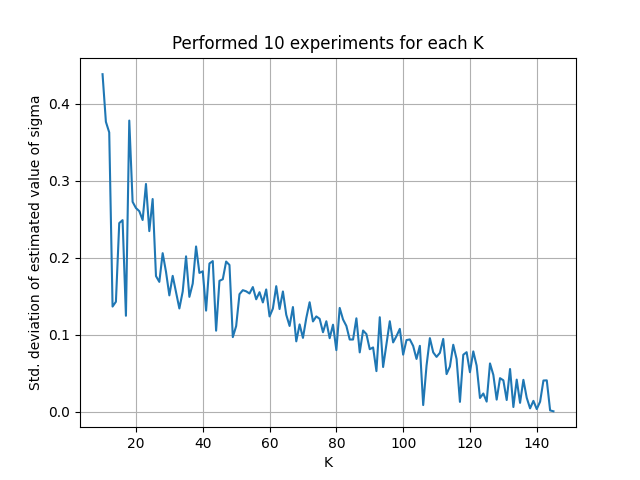
\includegraphics[width=\textwidth]{P1/sigma/stds_10.png}
        \caption[]{Std. deviation of $\hat{\sigma}_{MLE}$ observed}
    \end{subfigure}
    \caption{Number of iterations, $N = 10$}
\end{figure}
\newpage
\begin{figure}[H]
    \centering
    \begin{subfigure}[H]{0.49\textwidth}
        \centering
        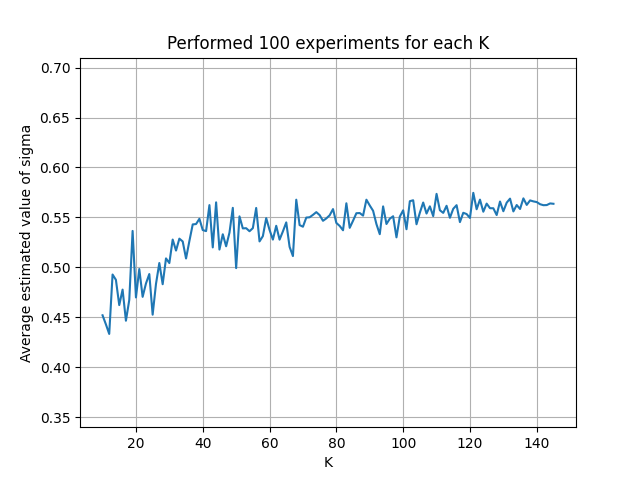
\includegraphics[width=\textwidth]{P1/sigma/avgs_100.png}
        \caption[]{Average value of $\hat{\sigma}_{MLE}$ observed}
    \end{subfigure}
    \begin{subfigure}[H]{0.49\textwidth}
        \centering
        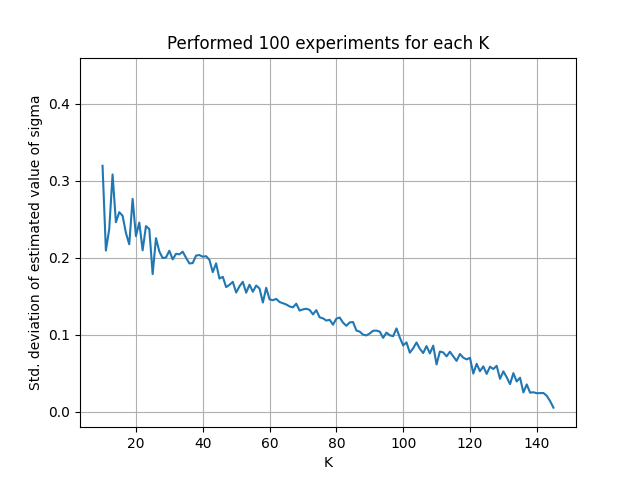
\includegraphics[width=\textwidth]{P1/sigma/stds_100.png}
        \caption[]{Std. deviation of $\hat{\sigma}_{MLE}$ observed}
    \end{subfigure}
    \caption{Number of iterations, $N = 100$}
\end{figure}
\vspace{0pt}
\begin{figure}[H]
    \centering
    \begin{subfigure}[H]{0.49\textwidth}
        \centering
        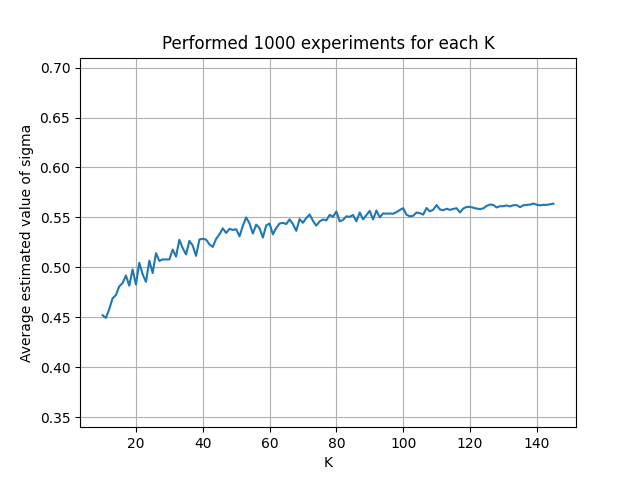
\includegraphics[width=\textwidth]{P1/sigma/avgs_1000.png}
        \caption[]{Average value of $\hat{\sigma}_{MLE}$ observed}
    \end{subfigure}
    \begin{subfigure}[H]{0.49\textwidth}
        \centering
        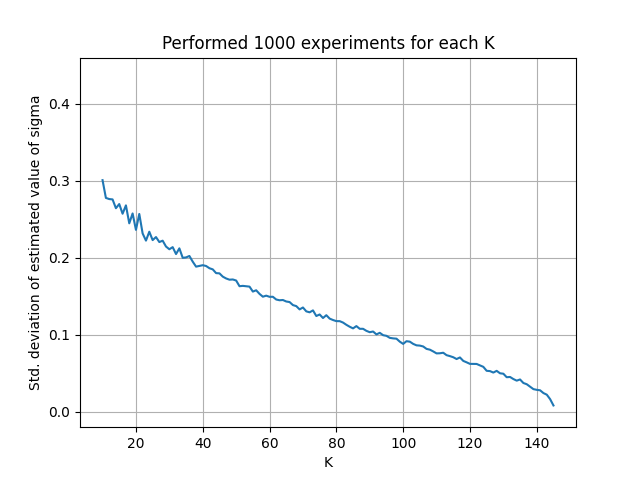
\includegraphics[width=\textwidth]{P1/sigma/stds_1000.png}
        \caption[]{Std. deviation of $\hat{\sigma}_{MLE}$ observed}
    \end{subfigure}
    \caption{Number of iterations, $N = 1000$}
\end{figure}

\subsection{Inference}
\begin{itemize}
    \item We can clearly observe that as $N$ increases, we are able to capture relation of variability of the estimates with $K$ very well.
    \item For large $N$, the expected value of estimate of $\mu$ for large $K$ is consistent (0.543).
    \item The expected value of estimate of $\sigma$ for large $N$ is dependent on $K$ because $\hat{\sigma^2}_{MLE}$ is proportional to a chi squared RV which has degrees of freedom dependent upon $K$.
    \item For small $N$, the average estimates for both $\mu$ and $\sigma$ vary more for small $K$. \\
          This can be explained by the large variance for small $K$.
\end{itemize}


\newpage
\section{Parameter estimation Problem 2}
\setcounter{figure}{0}
\subsection{Analysis of Age of death}
\begin{figure}[H]
    \centering
    \begin{subfigure}[H]{0.59\textwidth}
        \centering
        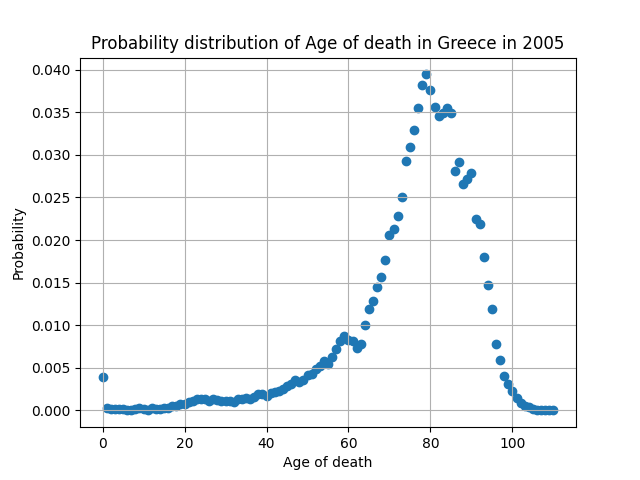
\includegraphics[width=\textwidth]{P2/plot.png}
        \caption[]{Probability distribution of Age of death in Greece in 2005}
    \end{subfigure}
    \caption{Analysis of Age of death in Greece in 2005}
\end{figure}

We can approximate the obtained probability mass function as $\mathrm{Binomial}(p, 110)$. \\
Here, the random variable is the age of death in Greece in 2005 which is a discrete random variable taking value in $\{0, \dots, 110\}$. \\

\subsection{Problem Description}
We assume that the age of people who died in Greece in 2005 follows $\mathrm{Binomial}(p, 110)$. \\
We are given a sample of age of death $a = (a_1, \dots, a_K)$ where $K$ is the sample size. \\
Estimated value of $p$ is $\hat{p}_{MLE} = \mathrm{mean}(a) / 110$.
We perform this experiment for $N$ iterations for a fixed $K$. \\
We analyze the observed estimated of $p$ for different $K$ and $N$. \\

\subsection{Generation of Sample}
\verb!mortality_Country.csv! contains total deaths per age interval, we cannot generate $a$ directly. \\
We extract probability distribution of age of death in Greece in 2005 for each age interval. \\
Our $K$-sized sample is a randomly generated $K$-sized list of ages with above obtained probability distribution. \\
We use function \verb!numpy.random.choice! with suitable arguments to obtain this sample. \\

\subsection{Results}
\begin{figure}[H]
    \centering
    \begin{subfigure}[H]{0.49\textwidth}
        \centering
        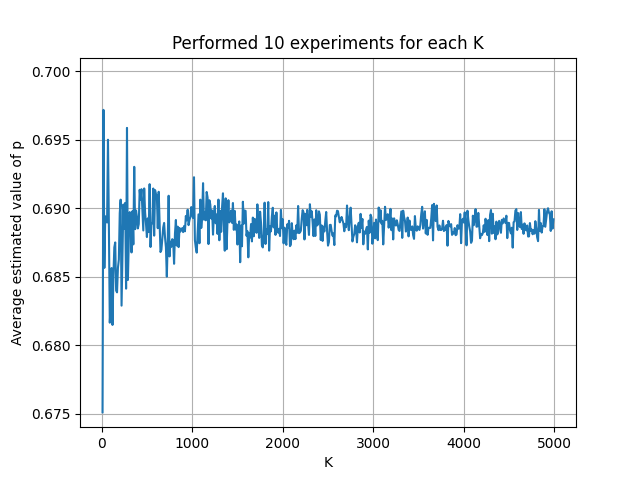
\includegraphics[width=\textwidth]{P2/avgs_10.png}
        \caption[]{Average value of $\hat{p}_{MLE}$ observed}
    \end{subfigure}
    \begin{subfigure}[H]{0.49\textwidth}
        \centering
        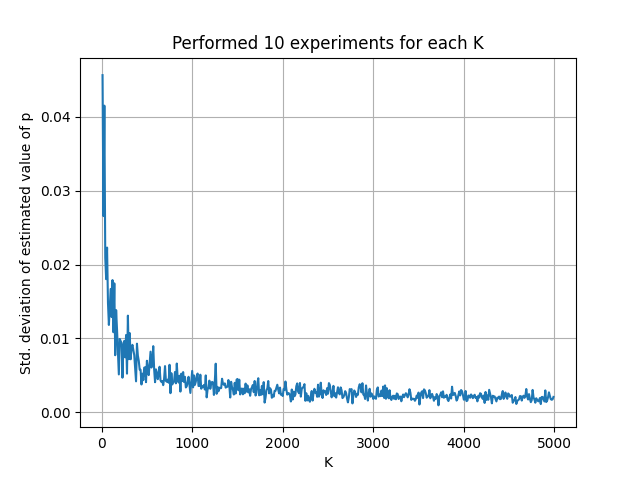
\includegraphics[width=\textwidth]{P2/stds_10.png}
        \caption[]{Std. deviation of $\hat{p}_{MLE}$ observed}
    \end{subfigure}
    \caption{Number of iterations, $N = 10$}
\end{figure}
\vspace{30pt}
\begin{figure}[H]
    \centering
    \begin{subfigure}[H]{0.49\textwidth}
        \centering`
        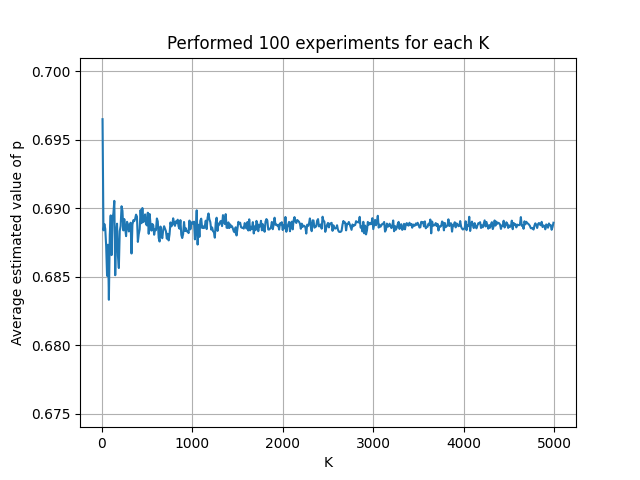
\includegraphics[width=\textwidth]{P2/avgs_100.png}
        \caption[]{Average value of $\hat{p}_{MLE}$ observed}
    \end{subfigure}
    \begin{subfigure}[H]{0.49\textwidth}
        \centering
        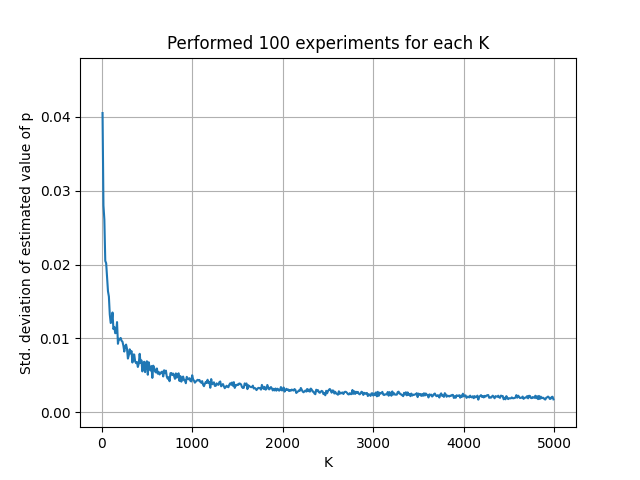
\includegraphics[width=\textwidth]{P2/stds_100.png}
        \caption[]{Std. deviation of $\hat{p}_{MLE}$ observed}
    \end{subfigure}
    \caption{Number of iterations, $N = 100$}
\end{figure}
\newpage
\begin{figure}[H]
    \centering
    \begin{subfigure}[H]{0.49\textwidth}
        \centering
        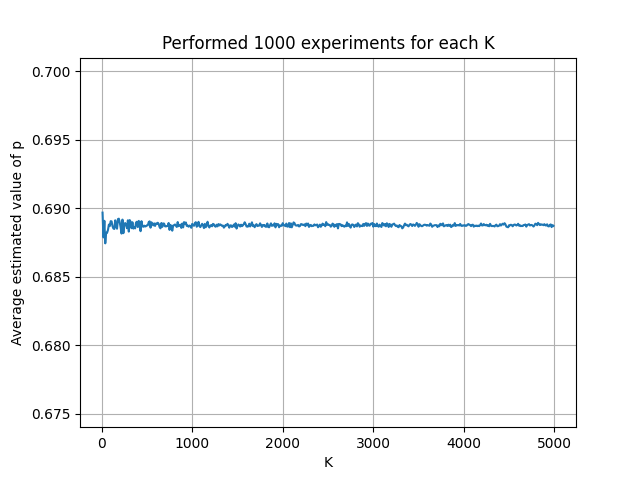
\includegraphics[width=\textwidth]{P2/avgs_1000.png}
        \caption[]{Average value of $\hat{p}_{MLE}$ observed}
    \end{subfigure}
    \begin{subfigure}[H]{0.49\textwidth}
        \centering
        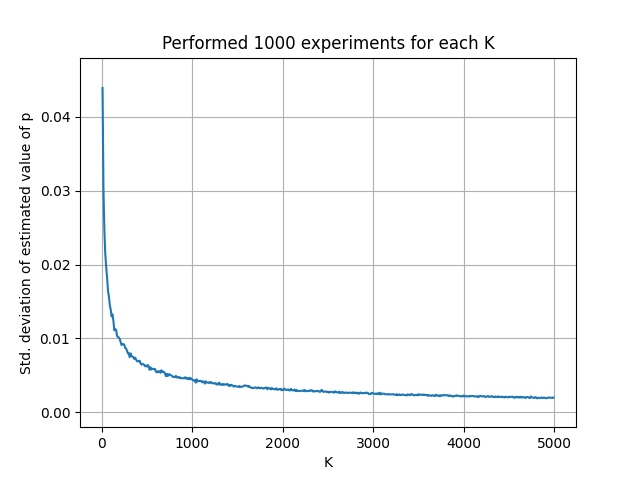
\includegraphics[width=\textwidth]{P2/stds_1000.png}
        \caption[]{Std. deviation of $\hat{p}_{MLE}$ observed}
    \end{subfigure}
    \caption{Number of iterations, $N = 1000$}
\end{figure}

\subsection{Inference}
\begin{itemize}
    \item We can clearly observe that as $N$ increases, we are able to capture relation of variability of the estimated value with $K$ very well.
    \item For large $N$, the expected value of estimate for all $K$ is consistent (almost 0.689). \\
          This sits well with law of large numbers.
    \item For small $N$, the average estimated varies more for small $K$. \\
          This can be explained by the large variance for small $K$.
\end{itemize}


\newpage
\section{Hypothesis Testing Problem 1}
\setcounter{figure}{0}
\subsection{Analysis of Gender Ratio}
\begin{figure}[H]
    \centering
    \begin{subfigure}[H]{0.49\textwidth}
        \centering
        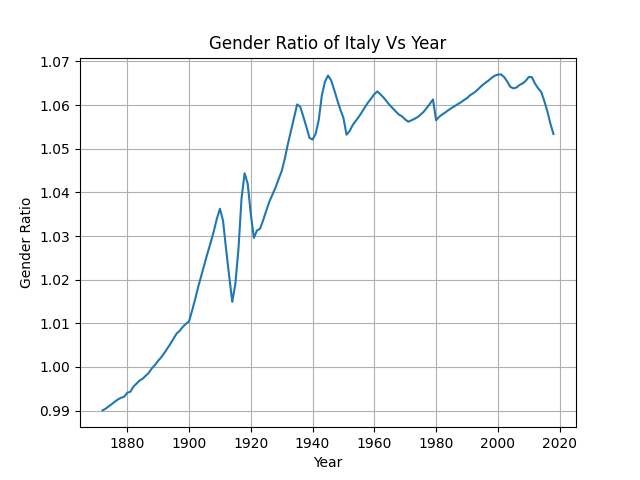
\includegraphics[width=\textwidth]{P3/plot_ita.png}
        \caption[]{Plot of Gender Ratio of Italy Vs Year}
    \end{subfigure}
    \begin{subfigure}[H]{0.49\textwidth}
        \centering
        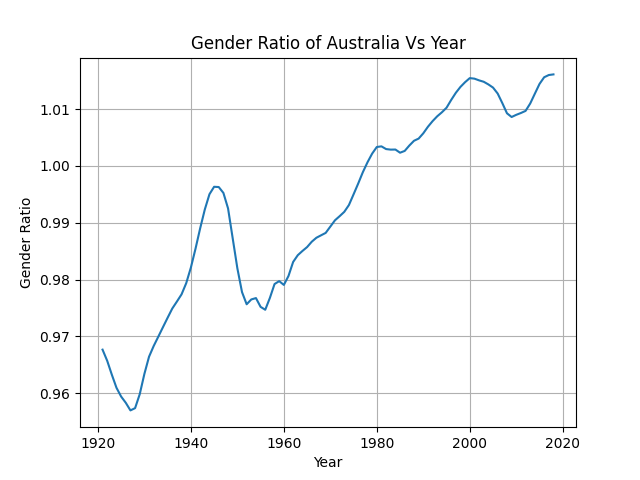
\includegraphics[width=\textwidth]{P3/plot_aus.png}
        \caption[]{Plot of Gender Ratio of Australia Vs Year}
    \end{subfigure}
    \caption{Analysis of Gender Ratio for Italy and Australia}
\end{figure}

From the above obtained plot, we can approximate gender ratios to be linear w.r.t. year. \\
Thus, we can conclude that gender ratio of Italy $\sim \mathrm{Uniform}[\theta_1 - \beta_1, \theta_1 + \beta_1]$. \\
Similarly, gender ratio of Australia $\sim \mathrm{Uniform}[\theta_2 - \beta_2, \theta_2 + \beta_2]$.

\subsection{Problem Description}
We assume that the gender ratio of Italy follows $\mathrm{Uniform}[\theta_1 - \beta_1, \theta_1 + \beta_1]$ distribution and that of Australia follows $\mathrm{Uniform}[\theta_2 - \beta_2, \theta_2 + \beta_2]$ distribution. \\
We are given a sample of gender ratio $\mathbf{r} = (r_1, \dots, r_K)$ where $K$ is the sample size which belongs to one of the above two mentioned distributions. \\
We devise a simple hypothesis: \\
H0: Country is Italy (i.e. $\theta$ = $\theta_1$) \\
H1: Country is Australia (i.e. $\theta = \theta_2$) \\
We perform following tests to accept/reject H0. \\
Test1: Reject H0 if $\mathrm{mean}(\mathbf{r}) < 1.0$ \\
Test2: Reject H0 if $\hat{\theta}_{MLE} = \dfrac{\mathrm{max}(\mathbf{r}) + \mathrm{min}(\mathbf{r})}{2} < 1.0$ \\
We perform this experiment for $2N$ iterations for a fixed $K$, choosing each distribution as the true distribution for $N$ iterations. \\
We analyze the observed values of Type I and Type II errors for the tests for different $K$ and $N$.

\subsection{Generation of Sample}
From \verb!population_Country.csv!, we determine year-wise gender ratio for Italy from 1872 to 2018 (list of size 147) and for Australia from 1921 to 2018 (list of size 98). \\
The gender ratios are computed as ratio of total female population (using \verb!Female2! column) and total male population (using \verb!Male2! column) for every year. \\
Our $K$-sized sample is a randomly chosen $K$-sized subset $(K \le 98)$ of one of the above obtained list. \\
For first $N$ iterations, we choose from list of Italy. For latter $N$ iterations, we choose from list of Australia. \\
We use function \verb!numpy.random.choice! with suitable arguments to obtain this sample. \\

\subsection{Results}
\begin{figure}[H]
    \centering
    \begin{subfigure}[H]{0.49\textwidth}
        \centering
        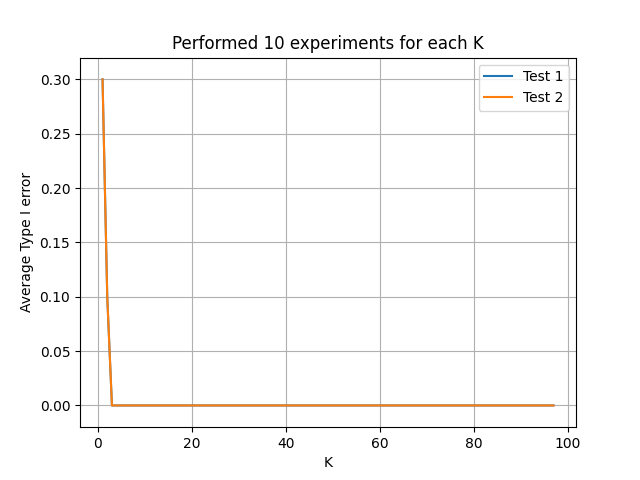
\includegraphics[width=\textwidth]{P3/type1_10.png}
        \caption[]{Average value of Type I error observed}
    \end{subfigure}
    \begin{subfigure}[H]{0.49\textwidth}
        \centering
        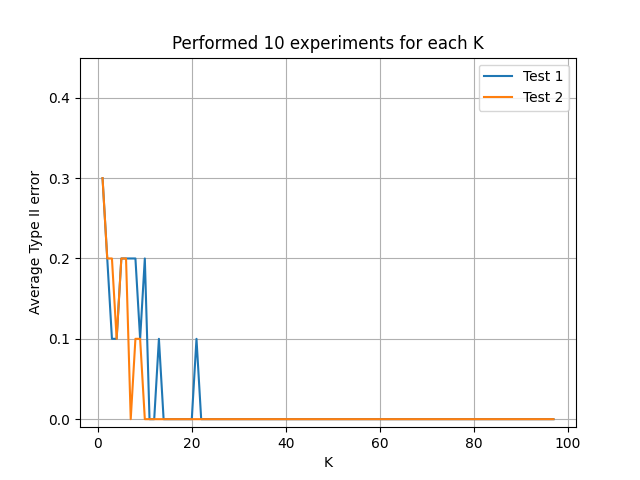
\includegraphics[width=\textwidth]{P3/type2_10.png}
        \caption[]{Average value of Type II error observed}
    \end{subfigure}
    \caption{Number of iterations for each side of hypothesis as truth, $N = 10$}
\end{figure}
\vspace{0pt}
\begin{figure}[H]
    \centering
    \begin{subfigure}[H]{0.49\textwidth}
        \centering
        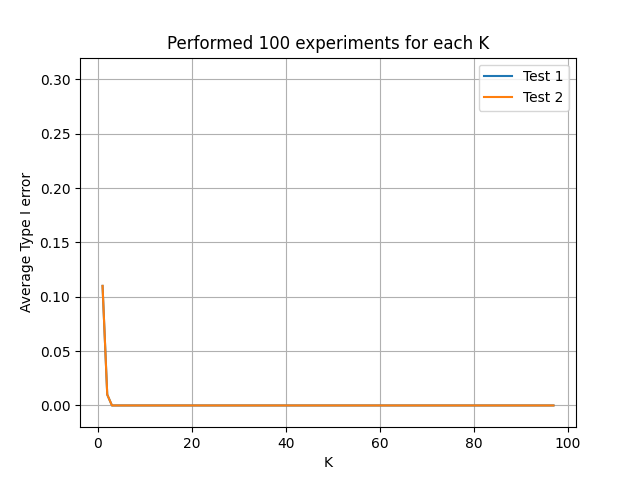
\includegraphics[width=\textwidth]{P3/type1_100.png}
        \caption[]{Average value of Type I error observed}
    \end{subfigure}
    \begin{subfigure}[H]{0.49\textwidth}
        \centering
        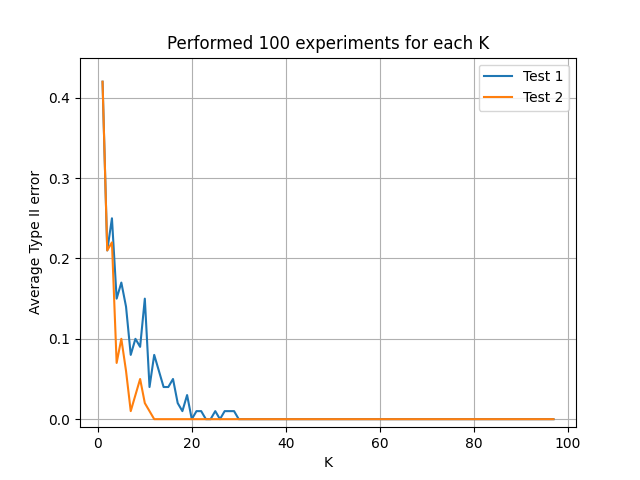
\includegraphics[width=\textwidth]{P3/type2_100.png}
        \caption[]{Average value of Type II error observed}
    \end{subfigure}
    \caption{Number of iterations for each side of hypothesis as truth, $N = 100$}
\end{figure}
\newpage
\begin{figure}[H]
    \centering
    \begin{subfigure}[H]{0.49\textwidth}
        \centering
        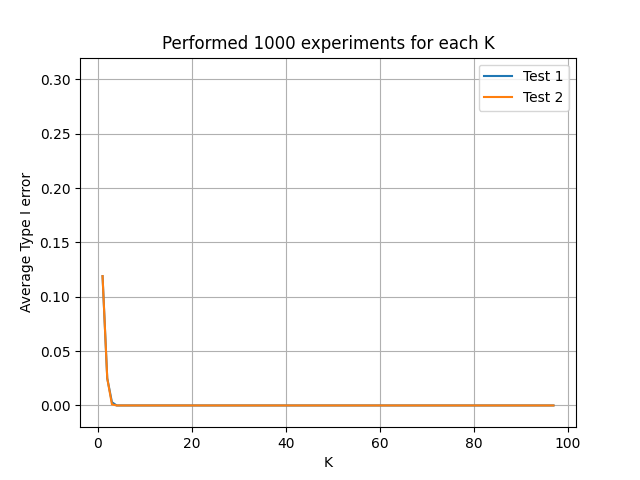
\includegraphics[width=\textwidth]{P3/type1_1000.png}
        \caption[]{Average value of Type I error observed}
    \end{subfigure}
    \begin{subfigure}[H]{0.49\textwidth}
        \centering
        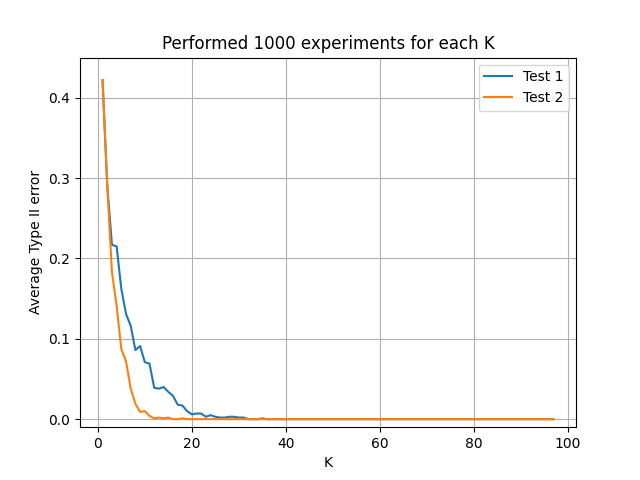
\includegraphics[width=\textwidth]{P3/type2_1000.png}
        \caption[]{Average value of Type II error observed}
    \end{subfigure}
    \caption{Number of iterations for each side of hypothesis as truth, $N = 1000$}
\end{figure}
\vspace{0pt}
\begin{figure}[H]
    \centering
    \begin{subfigure}[H]{0.49\textwidth}
        \centering
        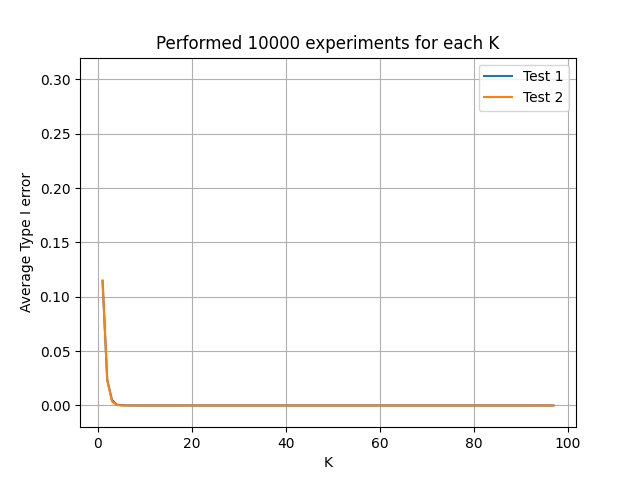
\includegraphics[width=\textwidth]{P3/type1_10000.png}
        \caption[]{Average value of Type I error observed}
    \end{subfigure}
    \begin{subfigure}[H]{0.49\textwidth}
        \centering
        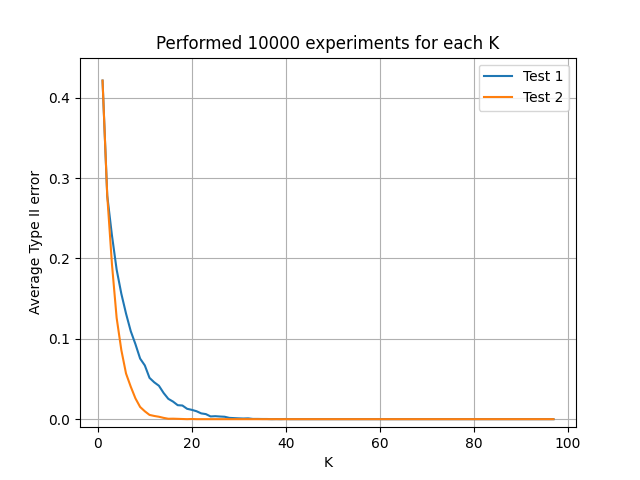
\includegraphics[width=\textwidth]{P3/type2_10000.png}
        \caption[]{Average value of Type II error observed}
    \end{subfigure}
    \caption{Number of iterations for each side of hypothesis as truth, $N = 10000$}
\end{figure}

\subsection{Inference}
\begin{itemize}
    \item As $N$ (i.e. the number of experiments for a given sample size) increases, we are able to capture relation of errors with $K$ (i.e the sample size) very well.
    \item The average value of Type I and Type II error for both tests decreases with the sample size for all values of N.
    \item Type I error is same for both tests. Type II error is less for Test 2. \\
          We can conclude that Test 2 is more powerful than Test 1.
\end{itemize}


\newpage
\section{Hypothesis Testing Problem 2}
\setcounter{figure}{0}
\subsection{Analysis of Population Growth Rate}
\begin{figure}[H]
    \centering
    \begin{subfigure}[H]{0.49\textwidth}
        \centering
        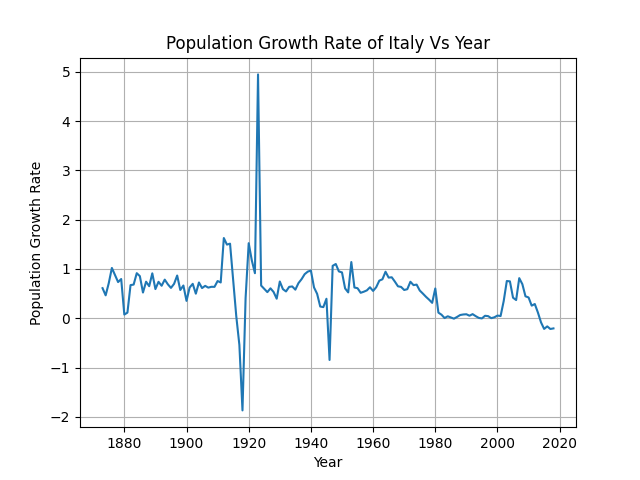
\includegraphics[width=\textwidth]{P4/plot_ita.png}
        \caption[]{Plot of Population Growth Rate of Italy Vs Year}
    \end{subfigure}
    \begin{subfigure}[H]{0.49\textwidth}
        \centering
        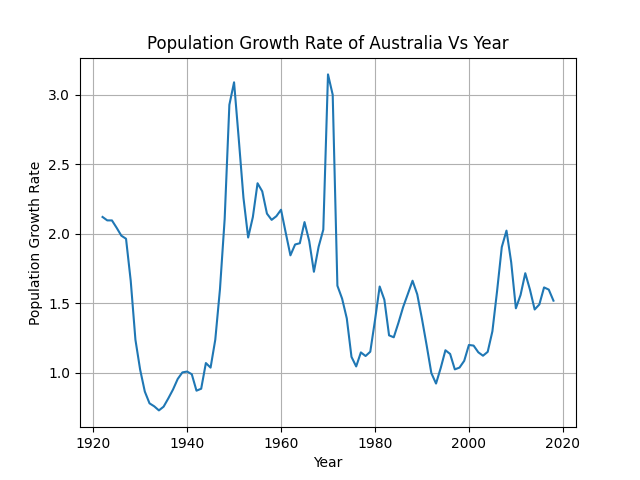
\includegraphics[width=\textwidth]{P4/plot_aus.png}
        \caption[]{Plot of Population Growth Rate of Australia Vs Year}
    \end{subfigure}
    \caption{Analysis of Population Growth Rate for Italy and Australia}
\end{figure}

From the above obtained plot, we can approximate population growth rate of Italy as a constant $\mu_1$ with zero-mean additive Gaussian noise, i.e. population growth rate of Italy $\sim \mathcal{N}(\mu_1, \sigma_1^2)$. \\
Similarly, population growth rate of Australia $\sim \mathcal{N}(\mu_2, \sigma_2^2)$.

\subsection{Problem Description}
We assume that the population growth rate of Italy follows $\mathcal{N}(\mu_1, \sigma_1^2)$ distribution and that of Australia follows $\mathcal{N}(\mu_2, \sigma_2^2)$ distribution. \\
We are given a sample of population growth rate $\mathbf{g} = (g_1, \dots, g_K)$ where $K$ is the sample size which belongs to one of the above two mentioned distributions. \\
We devise a simple hypothesis: \\
H0: Country is Italy (i.e. $\mu$ = $\mu_1$) \\
H1: Country is Australia (i.e. $\mu = \mu_2$) \\
We perform following test to accept/reject H0. \\
Test: Reject H0 if $\hat{\mu}_{MLE} = \mathrm{mean}(\mathbf{g}) > 1.2$ \\
We perform this experiment for $2N$ iterations for a fixed $K$, choosing each distribution as the true distribution for $N$ iterations. \\
We analyze the observed values of Type I and Type II errors for the test for different $K$ and $N$.

\subsection{Generation of Sample}
From \verb!population_Country.csv!, we determine year-wise population growth rate for Italy from 1872 to 2018 (list of size 147) and for Australia from 1921 to 2018 (list of size 98). \\
The population growth rates are computed as percentage change in population (using \verb!Total2! column) for every year. \\
Our $K$-sized sample is a randomly chosen $K$-sized subset $(K \le 98)$ of one of the above obtained list. \\
For first $N$ iterations, we choose from list of Italy. For latter $N$ iterations, we choose from list of Australia. \\
We use function \verb!numpy.random.choice! with suitable arguments to obtain this sample. \\

\subsection{Results}
\begin{figure}[H]
    \centering
    \begin{subfigure}[H]{0.49\textwidth}
        \centering
        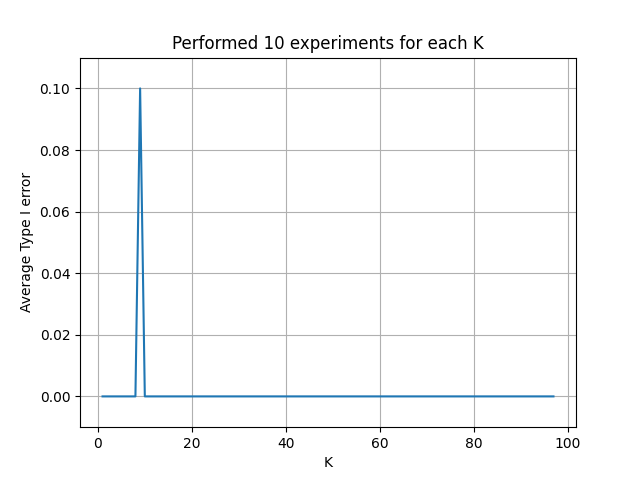
\includegraphics[width=\textwidth]{P4/type1_10.png}
        \caption[]{Average value of Type I error observed}
    \end{subfigure}
    \begin{subfigure}[H]{0.49\textwidth}
        \centering
        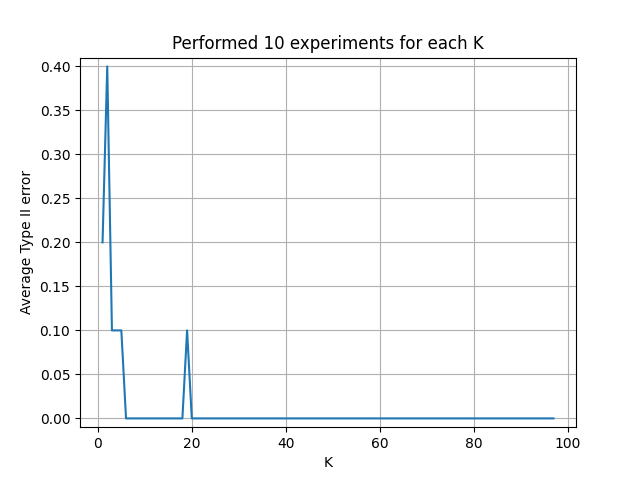
\includegraphics[width=\textwidth]{P4/type2_10.png}
        \caption[]{Average value of Type II error observed}
    \end{subfigure}
    \caption{Number of iterations for each side of hypothesis as truth, $N = 10$}
\end{figure}
\vspace{30pt}
\begin{figure}[H]
    \centering
    \begin{subfigure}[H]{0.49\textwidth}
        \centering
        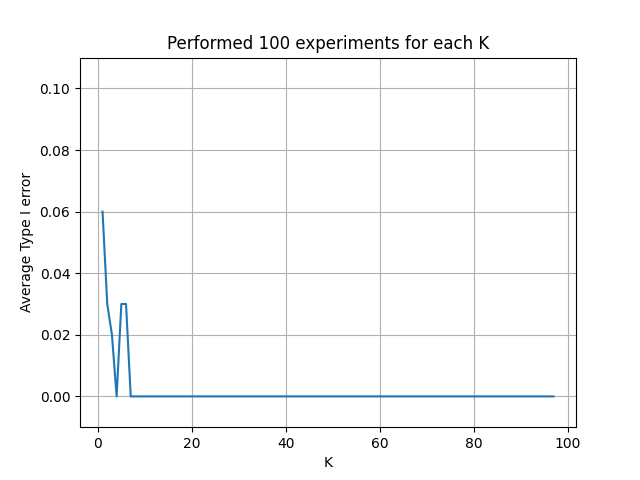
\includegraphics[width=\textwidth]{P4/type1_100.png}
        \caption[]{Average value of Type I error observed}
    \end{subfigure}
    \begin{subfigure}[H]{0.49\textwidth}
        \centering
        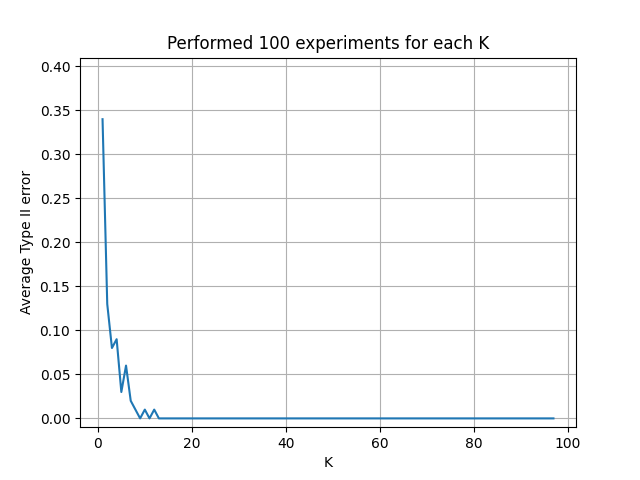
\includegraphics[width=\textwidth]{P4/type2_100.png}
        \caption[]{Average value of Type II error observed}
    \end{subfigure}
    \caption{Number of iterations for each side of hypothesis as truth, $N = 100$}
\end{figure}
\newpage
\begin{figure}[H]
    \centering
    \begin{subfigure}[H]{0.49\textwidth}
        \centering
        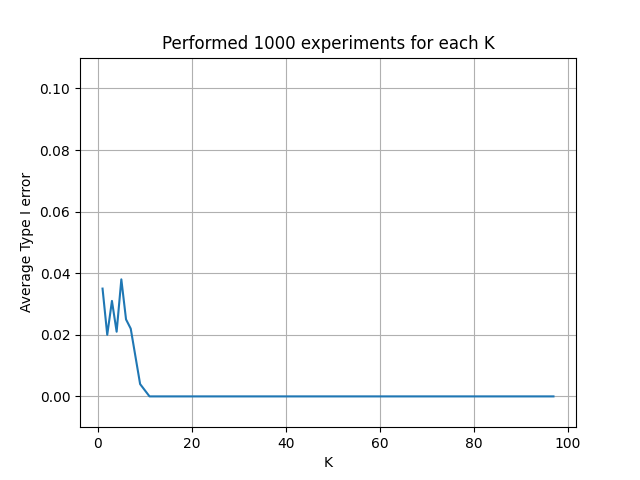
\includegraphics[width=\textwidth]{P4/type1_1000.png}
        \caption[]{Average value of Type I error observed}
    \end{subfigure}
    \begin{subfigure}[H]{0.49\textwidth}
        \centering
        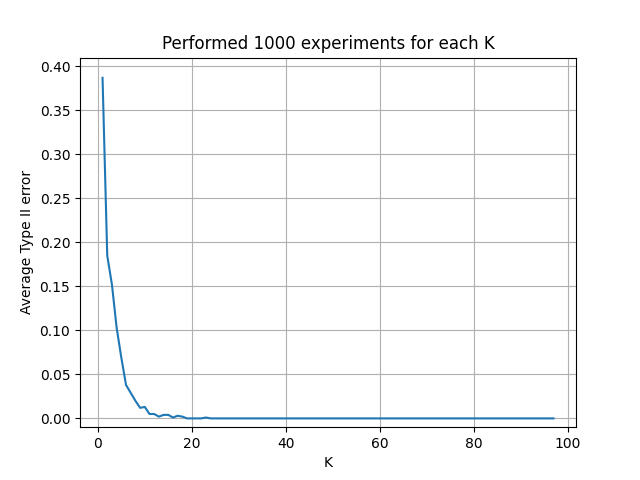
\includegraphics[width=\textwidth]{P4/type2_1000.png}
        \caption[]{Average value of Type II error observed}
    \end{subfigure}
    \caption{Number of iterations for each side of hypothesis as truth, $N = 1000$}
\end{figure}
\vspace{0pt}
\begin{figure}[H]
    \centering
    \begin{subfigure}[H]{0.49\textwidth}
        \centering
        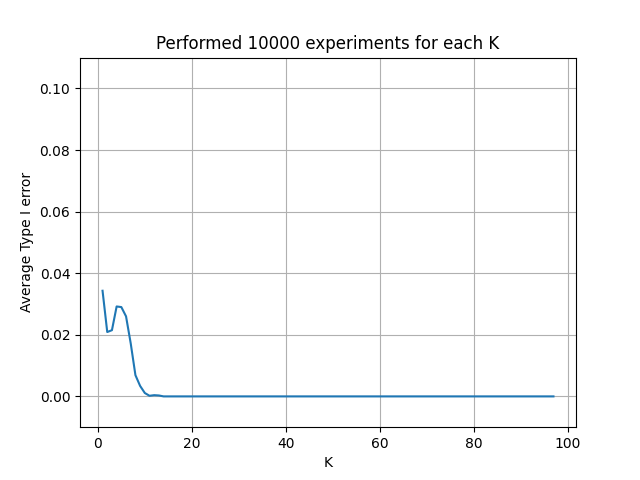
\includegraphics[width=\textwidth]{P4/type1_10000.png}
        \caption[]{Average value of Type I error observed}
    \end{subfigure}
    \begin{subfigure}[H]{0.49\textwidth}
        \centering
        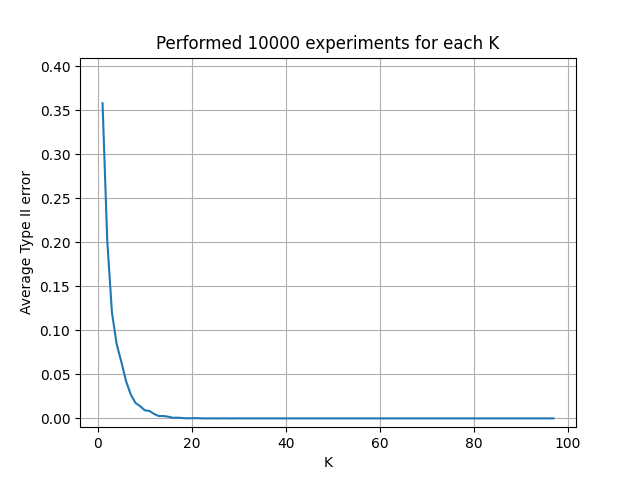
\includegraphics[width=\textwidth]{P4/type2_10000.png}
        \caption[]{Average value of Type II error observed}
    \end{subfigure}
    \caption{Number of iterations for each side of hypothesis as truth, $N = 10000$}
\end{figure}

\subsection{Inference}
\begin{itemize}
    \item As $N$ (i.e. the number of experiments for a given sample size) increases, we are able to capture relation of errors with $K$ (i.e the sample size) very well.
    \item The average value of Type I and Type II error decreases with the sample size for all values of N.
    \item The Type II error is more prevalent (i.e. has a higher probability of occurrence) for small values of $K$. At larger $K$ values, both errors are practically zero.
\end{itemize}



\end{document}
